\chapter{Конструкторский раздел}

В данном разделе описываются требования к разрабатываемому методу и программному обеспечению. Описываются основные этапы разрабатываемого метода и используемые алгоритмы. Также описывается архитектура используемой нейронной сети с модификациями для аэрофотоснимков. Выбирается порядок ядра интерполяции Ланцоша. 

\section{Требования к разрабатываемому методу}

К методу приведения аэрофотоснимков с различным разрешением к единому масштабу были сформулированы следующие требования:

\begin{itemize}[label=---]
    \item обеспечение повышения разрешения изображения до 4 раз включительно;
    \item поддержка изображений в форматах PNG и JPEG;
    \item возможность обработки цветовой модели RGB;
    \item обработка изображений с одинаковым соотношением сторон.
\end{itemize}

\section{Требования к программному обеспечению}

К программному обеспечению были сформулированы следующие требования:
\begin{itemize}[label=---]
    \item возможность загрузки нескольких изображений;
    \item возможность просмотра сведенных изображений;
    \item возможность скачивания результата сведения;
    \item возможность удаления изображений из сводимых. 
\end{itemize}

\section{Основные этапы разрабатываемого метода}

На рисунке~\ref{fig:cons:idefA1} представлена IDEF0 диаграмма первого уровня. 

\begin{figure}[H]
    \centering
    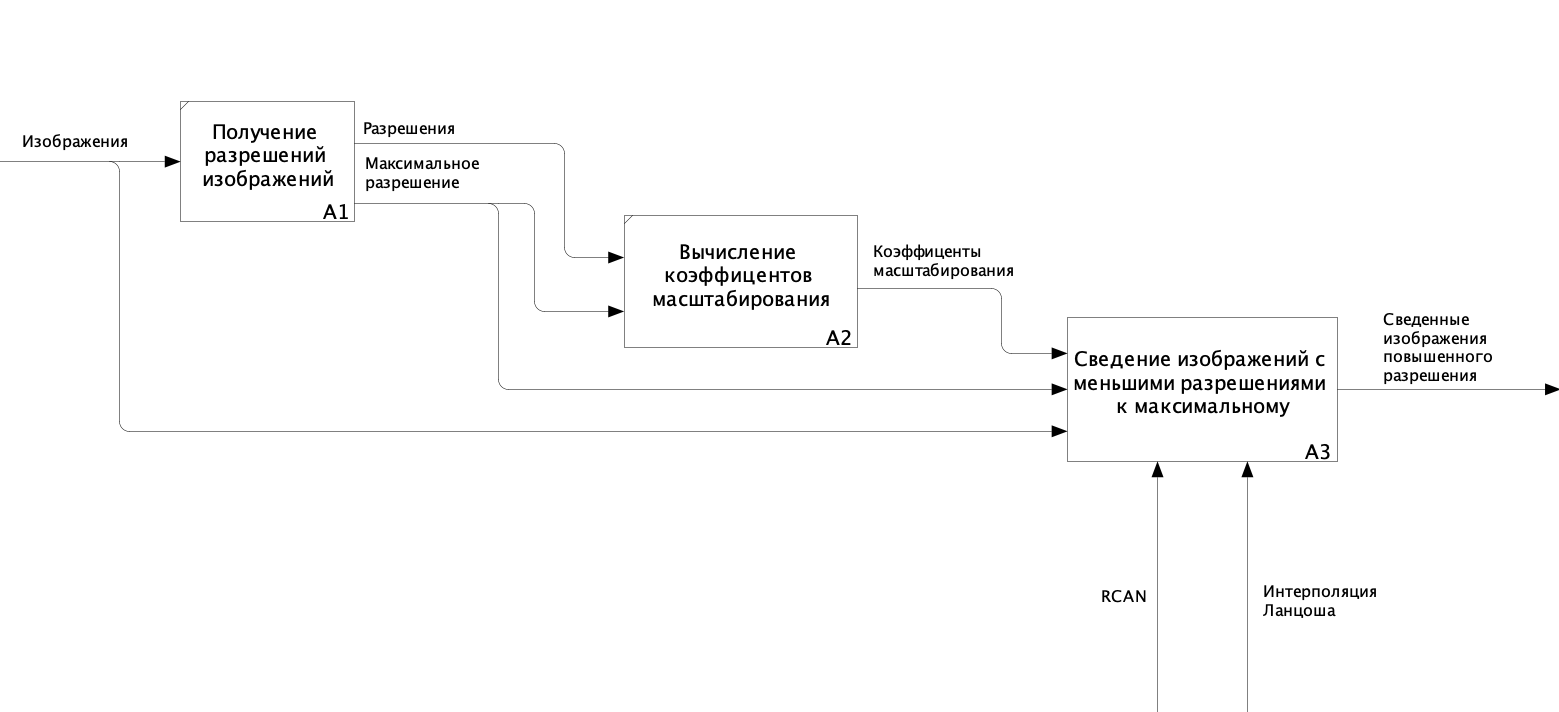
\includegraphics[width=1\linewidth]{images/construct/steps.png}
    \caption{IDEF0 диаграмма первого уровня}
    \label{fig:cons:idefA1}
\end{figure}

На вход методу подаются изображения разного разрешения со следующими ограничениями:

\begin{itemize}[label=---]
    \item цветовая модель RGB;
    \item изображения имеют одинаковое соотношение сторон;
    \item отношение максимального разрешения к минимальному не больше 4. 
\end{itemize}

Метод состоит из трех этапов:

\begin{enumerate}
    \item Первый этап получает с изображений их разрешения а также находит максимальное разрешение. 
    \item Второй этап вычисляет коэффициенты масштабирования, на которые надо увеличить исходные изображения до максимального разрешения. 
    \item Третий этап основываясь на коэффициентах сводит изображения к максимальному разрешению с использованием интерполяции Ланцоша и нейронной сети RCAN. 
\end{enumerate}

В результате работы метода возвращаются сведенные изображения высокого разрешения. 

\section{Алгоритм сведения изображений с меньшими разрешениями к максимальному}

На рисунке~\ref{fig:cons:scaler} представлена схема алгоритма сведения изображений с меньшими разрешениями к максимальному. 

\begin{figure}[H]
    \centering
    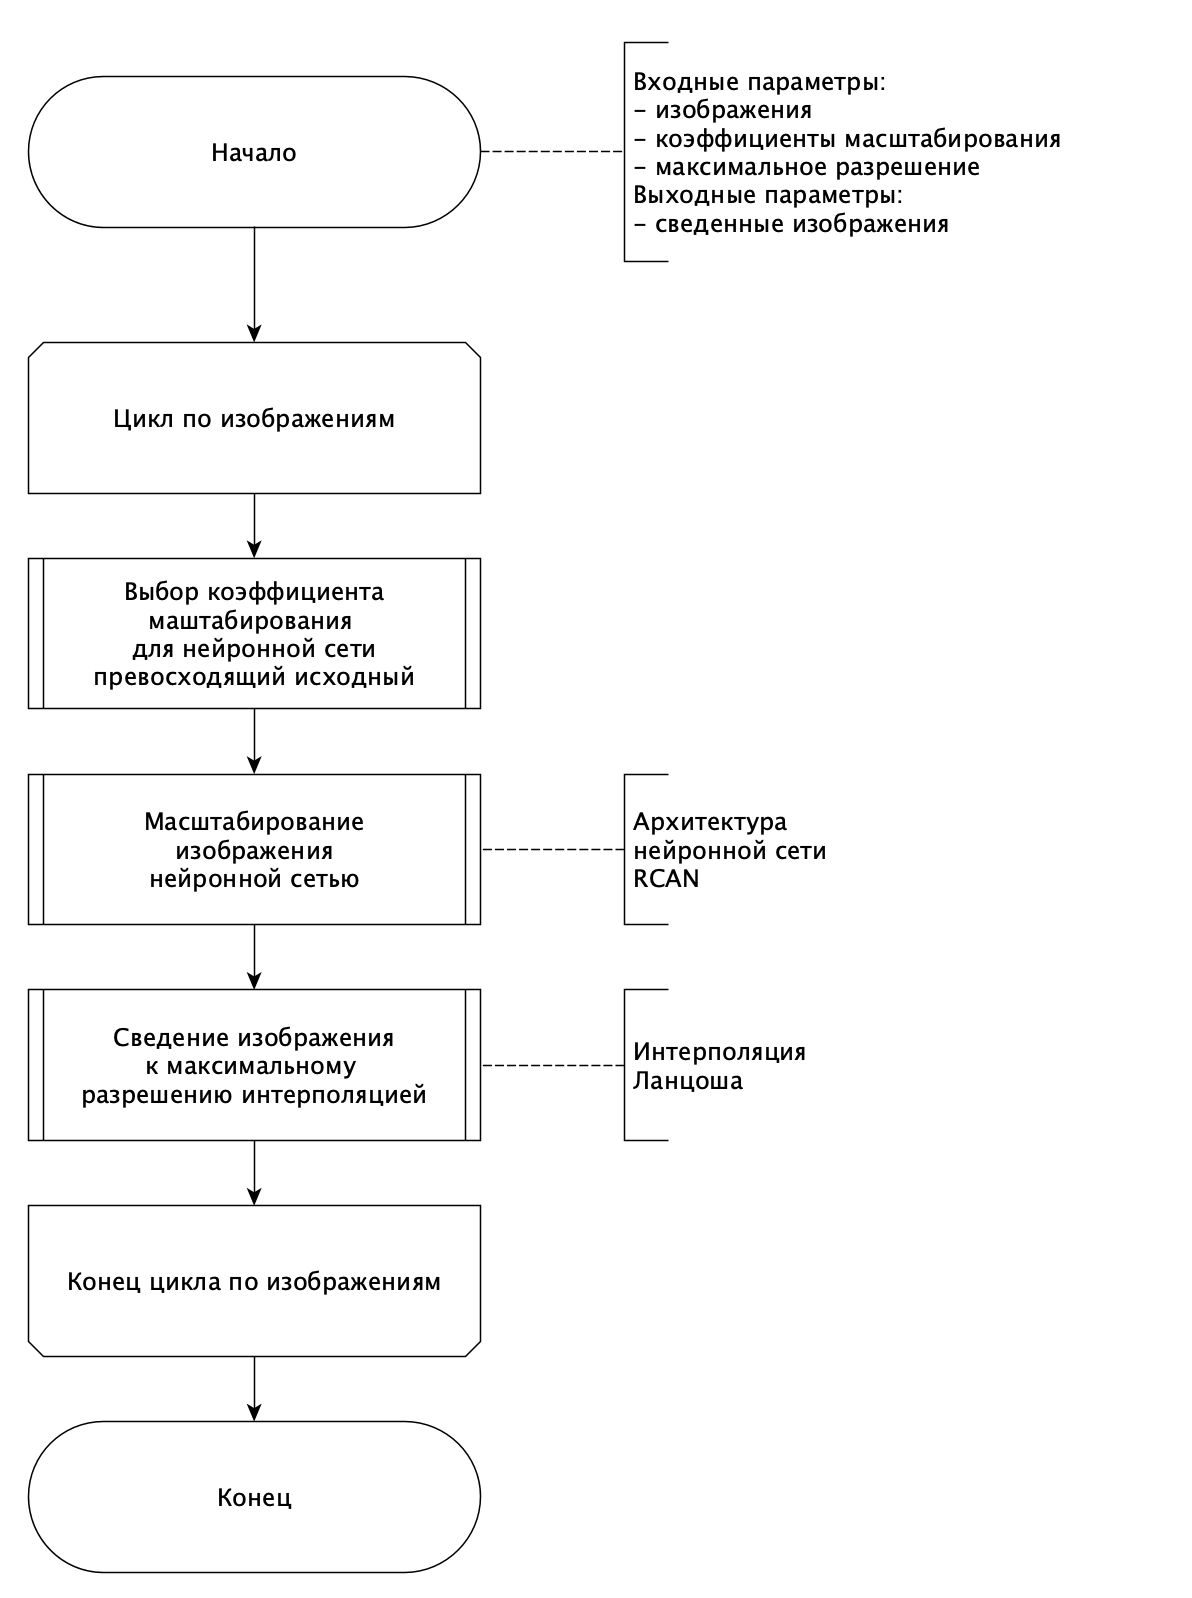
\includegraphics[width=0.6\linewidth]{images/construct/scaler.png}
    \caption{Схема алгоритма сведения изображений с меньшими разрешениями к максимальному}
    \label{fig:cons:scaler}
\end{figure}

Алгоритм итерируется по входным изображениям. Для каждого изображения выполняются следующие этапы:

\begin{enumerate}
    \item Выбор коэффициента масштабирования для нейронной сети. Коэффициент масштабирования, использующийся нейронной сетью превосходит исходный коэффициент масштабирования. 
    \item Изображение масштабируется нейронной сетью RCAN на найденный в предыдущем этапе коэффициент. 
    \item Изображение сверхразрешения, полученное нейронной сетью, с помощью интерполяции Ланцоша уменьшается до требуемого максимального разрешения. 
\end{enumerate}

В результате работы алгоритма возвращаются сведенные изображения высокого разрешения.

\section{Архитектура сети RCAN}

Архитектура RCAN представлена на рисунках~\ref{fig:cons:rcan}~---~\ref{fig:cons:rcab}. 

\begin{figure}[H]
    \centering
    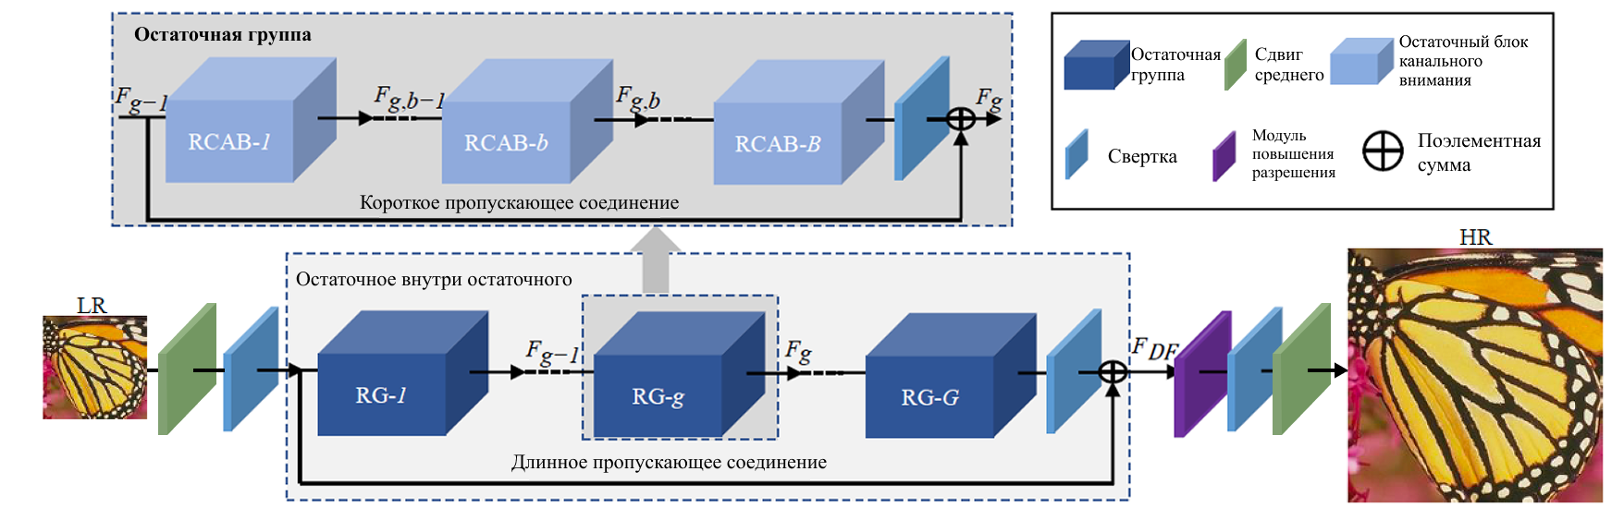
\includegraphics[width=1\linewidth]{images/construct/rcan_ru.png}
    \caption{Архитектура RCAN}
    \label{fig:cons:rcan}
\end{figure}

\begin{figure}[H]
    \centering
    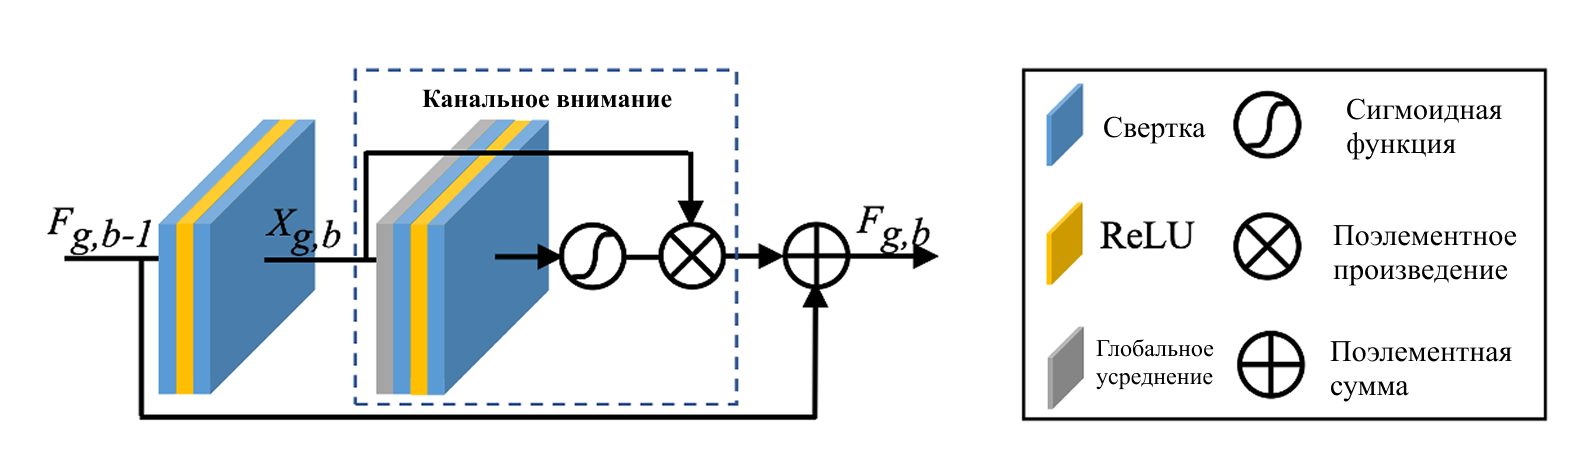
\includegraphics[width=0.8\linewidth]{images/construct/rcab_ru.png}
    \caption{Архитектура RCAB}
    \label{fig:cons:rcab}
\end{figure}

Сеть начинается со сверточного слоя, который извлекает начальные признаки из входного изображения низкого разрешения. Далее следует основная часть сети, построенная по принципу «остаточное внутри остаточного». Эта часть состоит из нескольких последовательных остаточных групп, каждая из которых включает множество остаточных блоков канального внимания RCAB.

Ключевым элементом архитектуры является блок RCAB. Внутри блока признаки последовательно проходят через два сверточных слоя с нелинейностью ReLU между ними. Затем применяется механизм канального внимания: глобальное усреднение признаков, после чего два полносвязных слоя с активациями ReLU и Сигмоидная функция вычисляют весовые коэффициенты для каждого канала. Эти веса перемножаются с исходными признаками, усиливая информативные каналы и подавляя менее значимые. Завершается блок остаточным соединением, суммирующим вход блока с полученным результатом.

В завершающей части сети признаки проходят через сверточный слой, после чего выполняется операция повышения разрешения субпиксельной сверткой. На выходе формируется изображение сверхвысокого разрешения.

В разрабатываемом методе будет использоваться 3 нейронные сети с архитектурой RCAN для повышения разрешения изображения в 2, 3 и 4 раза. Архитектура RCAN содержит 10 остаточных групп по 20 блоков RCAB в каждой.

Были выполнены следующие модификации архитектуры RCAN для  аэрофотоснимков:
\begin{enumerate}
    \item Реализована поддержка многомасштабного сверхразрешения посредством параметризации коэффициента масштабирования.
    
    \item Добавлена поддержка обработки данных с произвольным числом спектральных каналов.
    
    \item В архитектуру внедрен механизм нормализации входных данных на основе слоя, обеспечивающего вычитание средних значений цветовых каналов и последующее восстановление исходного диапазона интенсивностей.
\end{enumerate}

% \section{Алгоритм выбора коэффициента масштабирования нейронной сети}

% На рисунке~\ref{fig:cons:scaler} представлена схема алгоритма выбора коэффициента масштабирования нейронной сети.

% \begin{figure}[H]
%     \centering
%     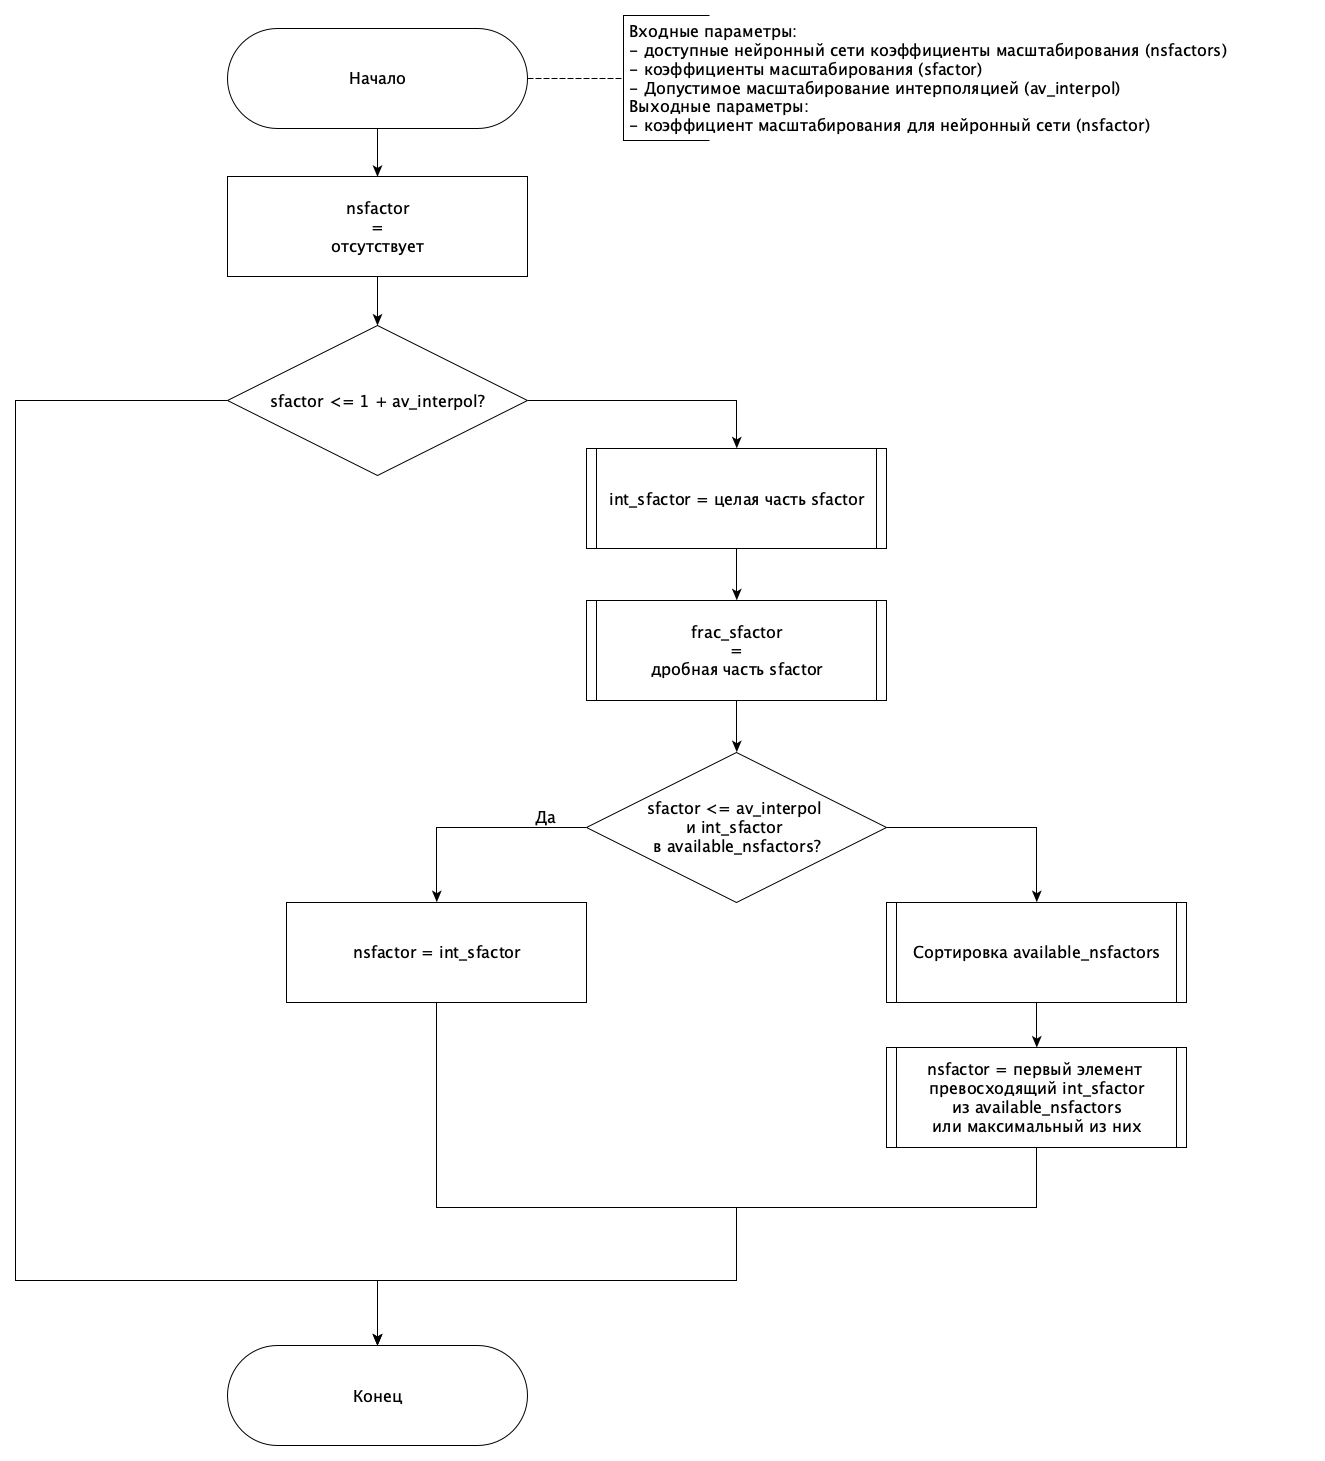
\includegraphics[width=0.8\linewidth]{images/construct/select.png}
%     \caption{Схема алгоритма выбора коэффициента масштабирования нейронной сети}
%     \label{fig:cons:selector}
% \end{figure}

\section{Интерполяция Ланцоша}

Ядро интерполяции Ланцоша порядка $n$ представлено в формуле~(\ref{f:c:lancoz}).

\begin{equation}
    L_n(x) = \begin{cases}
    \operatorname{sinc}(x) \cdot \operatorname{sinc}\left(\frac{x}{n}\right), & |x| < n, \\
    0, & |x| \geqslant n.
    \end{cases}
    \label{f:c:lancoz}
\end{equation}

Было проведено сравнение ядер 2, 3 и 4 порядка. Сравнение ядер представлено на рисунках~\ref{fig:cons:lpsnr}~---~\ref{fig:cons:lssim}. Сравнение проводилось на тестовом наборе Urban100. 

\begin{figure}[H]
    \centering
    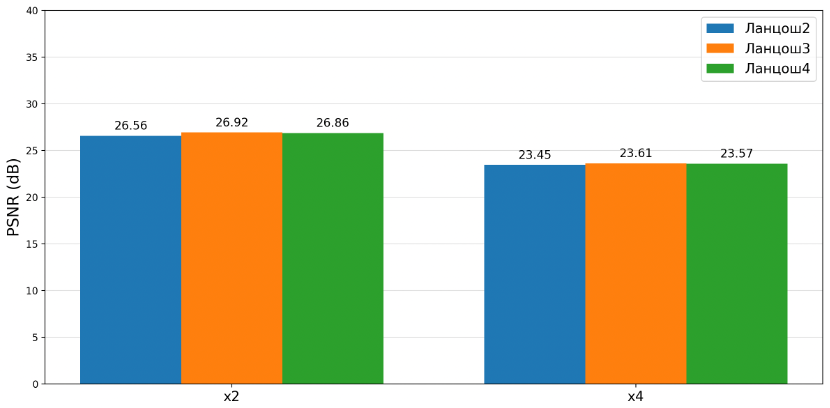
\includegraphics[width=0.9\linewidth]{images/construct/lan_psnr.png}
    \caption{Сравнение порядков Ядра Ланцоша по PSNR}
    \label{fig:cons:lpsnr}
\end{figure}

\begin{figure}[H]
    \centering
    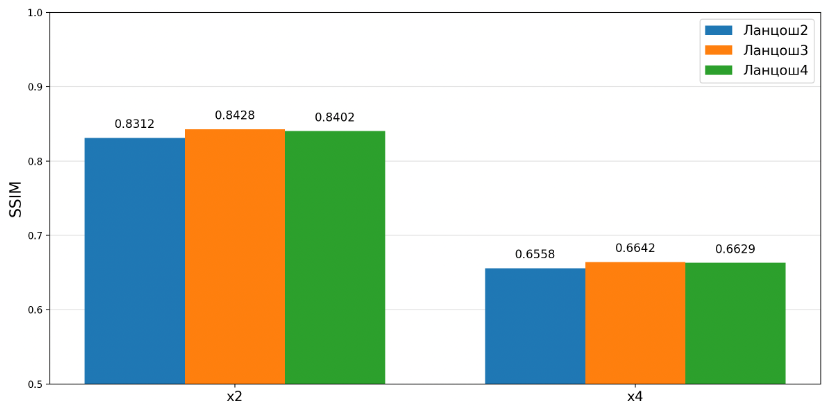
\includegraphics[width=0.9\linewidth]{images/construct/lan_ssim.png}
    \caption{Сравнение порядков Ядра Ланцоша по SSIM}
    \label{fig:cons:lssim}
\end{figure}

С ростом порядка ядра квадратично увеличивается количество участвующих в расчете пикселей, что напрямую влияет на вычислительную сложность интерполяции. Используемое количество пикселей в окне ядра порядка $n$ определяется как $(2n)^2$, поскольку ядро симметрично и учитывает окно размером $2n \times 2n$ пикселей. Из этого следует что ядра порядков 2, 3 и 4 используют 16, 36 и 64 пикселя соответственно. 

В разрабатываемом методе выбрано ядро Ланцоша третьего порядка. Данное решение обусловлено тем, что ядро третьего порядка превосходит остальные рассматриваемые порядки по качеству восстановления и при этом использует окно оптимального размера.

\section*{Вывод}
\addcontentsline{toc}{section}{Вывод}

В данном разделе были описаны требования к разрабатываемому методу и программному обеспечению. Были рассмотрены основные этапы разрабатываемого метода, представленные в виде IDEF0-диаграммы первого уровня, а также приведены схемы используемых алгоритмов. Подробно описана архитектура RCAN и предложенные ее модификации. На основе сравнительного анализа выбран порядок ядра интерполяции Ланцоша.